% --- shared colours (matplotlib tab10) ---
\definecolor{cblue}{RGB}{31,119,180}
\definecolor{cred}{RGB}{214,39,40}
\definecolor{cgreen}{RGB}{44,160,44}

% common picture options: 1 bit = 0.042 cm on both axes (square aspect)
\tikzset{bitsec/.style={x=0.042cm,y=0.042cm,font=\small}}

%======================================================================
% PANEL 1 :  log t  vs  log eps   (advantage view)  --  SEARCH / linear
%======================================================================
\newcommand{\panelEpsSearch}{%
  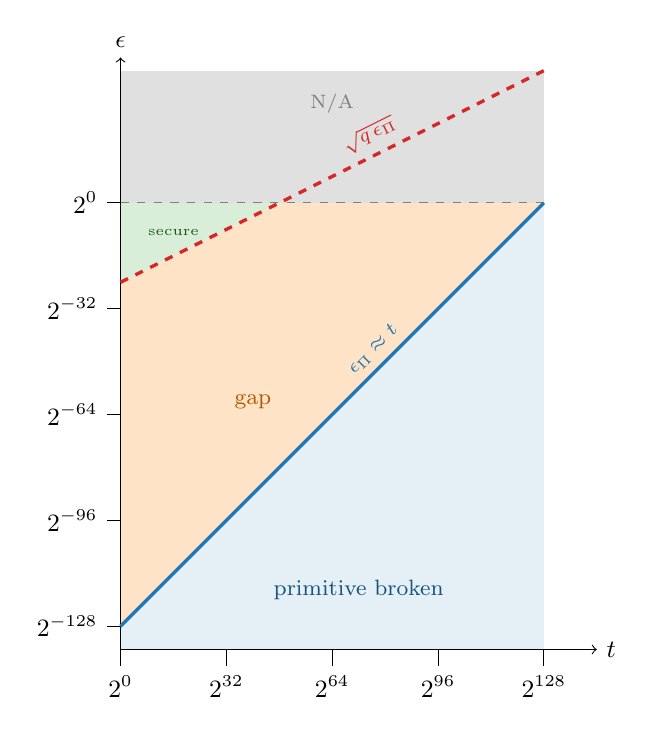
\begin{tikzpicture}[bitsec]
    \def\n{128}
    \fill[black!12]  (0,0) -- (0,40) -- (\n,40) -- (\n,0) -- cycle;
    \fill[cblue!12]  (0,-\n) -- (\n,0) -- (\n,-135) -- (0,-135) -- cycle;
    \fill[orange!22] (0,-\n) -- (\n,0) -- (48,0) -- (0,-24) -- cycle;   % gap
    \fill[cgreen!18] (0,0) -- (0,-24) -- (48,0) -- cycle;              % secure wedge
    \draw[->] (0,-135) -- (0,44) node[above] {$\epsilon$};
    \draw[->] (0,-135) -- ({\n+16},-135) node[right] {$t$};
    \foreach \x in {0,32,64,96,128} \draw (\x,-135)--(\x,-140) node[below] {$2^{\x}$};
    \foreach \y in {0,-32,-64,-96,-128} \draw (0,\y)--(-4,\y) node[left] {$2^{\y}$};
    \draw[gray,dashed] (0,0) -- (\n,0);
    \node[gray,font=\scriptsize] at ({0.5*\n},30) {N/A};
    \draw[cblue,very thick] (0,-\n) -- (\n,0);
    \draw[cred,very thick,dashed] (0,-24) -- (\n,40);            % sqrt(q*eps) = 2^{tau/2-24}
    \node[cblue,rotate=45,anchor=south,font=\scriptsize] at (80,-48) {$\epsilon_\Pi \approx t$};
    \node[cred,rotate=26.57,anchor=south,font=\scriptsize] at (78,15) {$\sqrt{q\,\epsilon_\Pi}$};
    \node[cgreen!55!black,align=center,font=\tiny] at (16,-9) {secure};
    \node[orange!70!black,align=center,font=\footnotesize] at (40,-60) {gap};
    \node[cblue!70!black,align=center,font=\footnotesize] at (72,-117) {primitive broken};
  \end{tikzpicture}
}

%======================================================================
% PANEL 2 :  log t  vs  log eps   --  GROVER / collision
%======================================================================
\newcommand{\panelEpsGrover}{%
  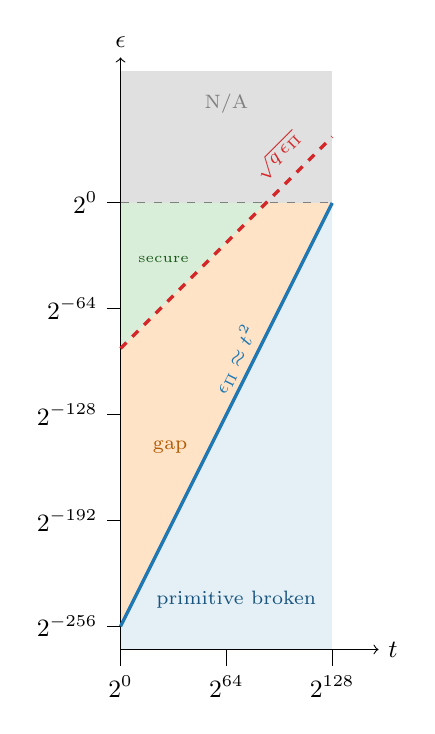
\begin{tikzpicture}[bitsec]
    \def\n{128}\def\m{64}
    \fill[black!12]  (0,0) -- (0,40) -- (\m,40) -- (\m,0) -- cycle;
    \fill[cblue!12]  (0,-\n) -- (\m,0) -- (\m,-135) -- (0,-135) -- cycle;
    \fill[orange!22] (0,-\n) -- (\m,0) -- (44,0) -- (0,-44) -- cycle;   % gap
    \fill[cgreen!18] (0,0) -- (0,-44) -- (44,0) -- cycle;              % secure wedge
    \draw[->] (0,-135) -- (0,44) node[above] {$\epsilon$};
    \draw[->] (0,-135) -- ({\m+14},-135) node[right] {$t$};
    \foreach \x in {0,64,128} \draw ({\x/2},-135)--({\x/2},-140) node[below] {$2^{\x}$};
    \foreach \y in {0,-64,-128,-192,-256} \draw (0,{\y/2})--(-4,{\y/2}) node[left] {$2^{\y}$};
    \draw[gray,dashed] (0,0) -- (\m,0);
    \node[gray,font=\scriptsize] at (32,30) {N/A};
    \draw[cblue,very thick] (0,-\n) -- (\m,0);
    \draw[cred,very thick,dashed] (0,-44) -- (\m,20);            % sqrt(q*eps) = 2^{tau-88}
    \node[cblue,rotate=63.43,anchor=south,font=\scriptsize] at (40,-50) {$\epsilon_\Pi \approx t^2$};
    \node[cred,rotate=45,anchor=south,font=\scriptsize] at (52,10) {$\sqrt{q\,\epsilon_\Pi}$};
    \node[cgreen!55!black,align=center,font=\tiny] at (13,-17) {secure};
    \node[orange!70!black,align=center,font=\scriptsize] at (15,-74) {gap};
    \node[cblue!70!black,align=center,font=\scriptsize] at (35,-120) {primitive broken};
  \end{tikzpicture}
}

%======================================================================
% PANEL 3 :  t  vs  kappa   (bit-security view)  --  SEARCH / linear
%======================================================================
\newcommand{\panelKapSearch}{%
  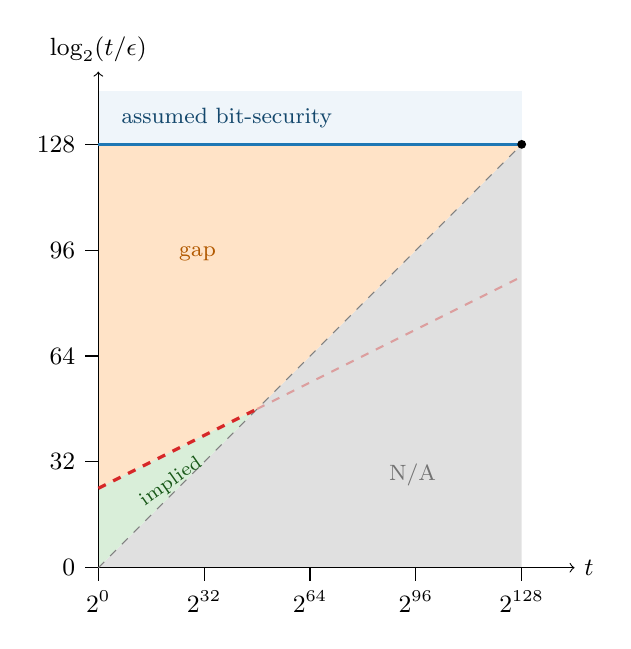
\begin{tikzpicture}[bitsec]
    \def\n{128}
    \fill[cblue!7]   (0,\n) -- (0,{\n+16}) -- (\n,{\n+16}) -- (\n,\n) -- cycle;
    \fill[black!12]  (0,0) -- (\n,\n) -- (\n,0) -- cycle;
    \fill[orange!22] (0,24) -- (48,48) -- (\n,\n) -- (0,\n) -- cycle;   % gap
    \fill[cgreen!18] (0,0) -- (0,24) -- (48,48) -- cycle;              % implied wedge (24-bit)
    \draw[->] (0,0) -- (0,{\n+22}) node[above] {$\log_2(t/\epsilon)$};
    \draw[->] (0,0) -- ({\n+16},0) node[right] {$t$};
    \foreach \x in {0,32,64,96,128} \draw (\x,0)--(\x,-4) node[below] {$2^{\x}$};
    \foreach \y in {0,32,64,96,128} \draw (0,\y)--(-4,\y) node[left] {$\y$};
    \draw[gray,dashed] (0,0) -- (\n,\n);
    \draw[cblue,very thick] (0,\n) -- (\n,\n);
    \draw[cred,very thick,dashed] (0,24) -- (48,48);            % kappa_A = tau/2+24
    \draw[cred,thick,dashed,opacity=0.35] (48,48) -- (\n,88);
    \fill (\n,\n) circle (1.6pt);
    \node[cblue!60!black,anchor=west,font=\footnotesize] at (4,{\n+8}) {assumed bit-security};
    \node[orange!70!black,font=\footnotesize] at (30,95) {gap};
    \node[cgreen!55!black,rotate=35,font=\scriptsize] at (22,26) {implied};
    \node[black!55,align=center,font=\footnotesize] at (95,28) {N/A};
  \end{tikzpicture}
}

%======================================================================
% PANEL 4 :  t  vs  kappa   --  GROVER / collision
%======================================================================
\newcommand{\panelKapGrover}{%
  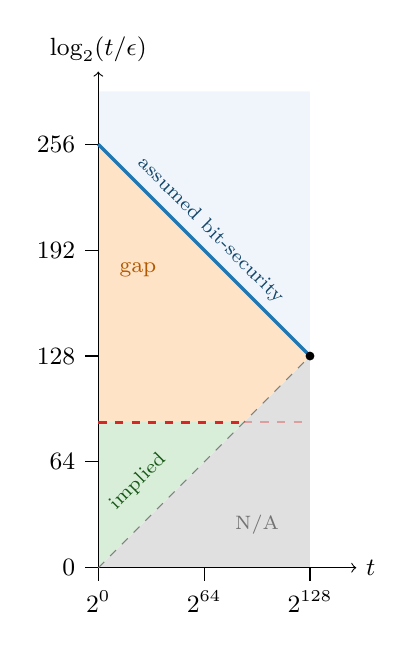
\begin{tikzpicture}[bitsec]
    \def\n{128}\def\m{64}
    \fill[cblue!7]   (0,\n) -- (0,{\n+16}) -- (\m,{\n+16}) -- (\m,\m) -- cycle;
    \fill[black!12]  (0,0) -- (\m,\m) -- (\m,0) -- cycle;
    \fill[orange!22] (0,44) -- (44,44) -- (\m,\m) -- (0,\n) -- cycle;   % gap
    \fill[cgreen!18] (0,0) -- (0,44) -- (44,44) -- cycle;              % implied wedge (88-bit)
    \draw[->] (0,0) -- (0,{\n+22}) node[above] {$\log_2(t/\epsilon)$};
    \draw[->] (0,0) -- ({\m+14},0) node[right] {$t$};
    \foreach \x in {0,64,128} \draw ({\x/2},0)--({\x/2},-4) node[below] {$2^{\x}$};
    \foreach \y in {0,64,128,192,256} \draw (0,{\y/2})--(-4,{\y/2}) node[left] {$\y$};
    \draw[gray,dashed] (0,0) -- (\m,\m);
    \draw[cblue,very thick] (0,\n) -- (\m,\m);
    \draw[cred,very thick,dashed] (0,44) -- (44,44);            % kappa_A = 88 (flat)
    \draw[cred,thick,dashed,opacity=0.35] (44,44) -- (\m,44);
    \fill (\m,\m) circle (1.6pt);
    \node[cblue!60!black,rotate=-45,anchor=south,font=\scriptsize] at (30,98) {assumed bit-security};
    \node[orange!70!black,font=\footnotesize] at (12,90) {gap};
    \node[cgreen!55!black,rotate=45,font=\scriptsize] at (12,26) {implied};
    \node[black!55,font=\scriptsize] at (48,13) {N/A};
  \end{tikzpicture}
}

%%% Invoking the Panels as Sub-Figures %%%
% Fixed scale + tabular  =>  Grover panel is literally half as wide,
% and the two x-axes align on a common baseline automatically.
%\begin{tabular}{@{}c@{\hspace{3em}}c@{}}
%  \panelEpsSearch & \panelEpsGrover\\[3pt]
%  {\small (a) Attack space if best primitive attack $=$ brute-force} & {\small (b) Attack space if best primitive attack $=$ Grover}\\[8pt]
%  \panelKapSearch & \panelKapGrover\\[3pt]
%  {\small (c) Bit security if best primitive attack $=$ brute-force} & {\small (d) Bit security if best primitive attack $=$ Grover}\\
%\end{tabular}

\begin{tabular}{@{}c@{\hspace{3em}}c@{}}
  \panelcap{\panelEpsSearch}{
    %(a) Possible attacks if best attack against the
    %primitive scales linearly with time (brute-force)
    (a) Ruled-out attacks if the best attack on the primitive scales
    \emph{linearly} (brute-force)
  }
& \panelcap{\panelEpsGrover}{
    (b) vs.\ \emph{quadratically} (birthday/Grover)
  }\\[30pt]
  \panelcap{\panelKapSearch}{
    %(c) Bit security if best primitive attack $=$ brute-force
    (c) Bit security if the best attack on the primitive scales
    \emph{linearly} (brute-force)
  }
& \panelcap{\panelKapGrover}{
    (d) vs.\ \emph{quadratically} (birthday/Grover)
  }\\
\end{tabular}
